\documentclass[conference]{IEEEtran}
\usepackage{amsmath,amssymb,graphicx,booktabs,url}
\usepackage{iftex}
\ifXeTeX
\usepackage{fontspec}
\setmainfont{NimbusRoman}[Path=fonts/,Extension=.otf,UprightFont=*-Regular,BoldFont=*-Bold,ItalicFont=*-Italic,BoldItalicFont=*-BoldItalic]
\setsansfont{NimbusSans}[Path=fonts/,Extension=.otf,UprightFont=*-Regular,BoldFont=*-Bold,ItalicFont=*-Italic,BoldItalicFont=*-BoldItalic]
\setmonofont{NimbusMonoPS}[Path=fonts/,Extension=.otf,UprightFont=*-Regular,BoldFont=*-Bold,ItalicFont=*-Italic,BoldItalicFont=*-BoldItalic]
\else\usepackage[T1]{fontenc}\fi
\usepackage[hidelinks]{hyperref}
% The public model package is committed with frozen provenance. Add the personal video after upload.
\newcommand{\ModelDownloadLink}{\href{https://raw.githubusercontent.com/M-Shaffan-Ahmad/GENAI_ImageSketchGenerator/main/artifacts/trained_models.zip}{Public ONNX model package (repository artifacts/)}}
\newcommand{\DemoVideoLink}{Pending personal recording and unlisted YouTube upload}
\newcommand{\StitchEvidenceStatus}{Supplied export preserved and implemented; see Fig.~\ref{fig:stitch}}

\IfFileExists{generated/test_numbers.tex}{\newcommand{\TestAccuracy}{0.9736}
\newcommand{\TestFOne}{0.9590}
}{\newcommand{\TestAccuracy}{pending}\newcommand{\TestFOne}{pending}}
\title{Universal, Hard-Routed and Soft-Mixture Restoration with Style-Conditioned Sketch Generation on Flowers102}
\author{\IEEEauthorblockN{Muhammad Shaffan Ahmad}
\IEEEauthorblockA{23i-0673, Section A\\CS4065 / Generative AI\\FAST NUCES}}
\begin{document}
\maketitle
\begin{abstract}
This project implements four related image systems: a universal convolutional autoencoder, hard routing between corruption specialists, a differentiable soft mixture with an identity branch, and a style-conditioned sketch generator. Flowers102 supplies the photographic domain; three deterministic image-processing algorithms supply paired sketch targets. Development splits group image duplicates and keep all sketch styles of a photograph together. Optuna studies and MLflow records support validation-based selection, and frozen models are evaluated on the official test photographs. Validation shows that specialization and soft blending improve corrupted-image restoration, while mild blur, missing-region detail and clean-image preservation remain difficult. Test sketch SSIM is 0.902 for pencil, 0.527 for ink and 0.818 for charcoal, indicating unequal target approximation across styles. All seven inference graphs are exported to ONNX and integrated into a React/FastAPI application. The report distinguishes measured quality, numerical export parity, deployment verification and remaining account-dependent submission evidence; it makes no claim of novel architecture or perfect restoration.
\end{abstract}
\begin{IEEEkeywords}image restoration, autoencoder, mixture of experts, conditional GAN, Flowers102, ONNX\end{IEEEkeywords}

\section{Introduction}
Image restoration must remove corruption without unnecessarily changing useful information. A single compressed model can handle several perturbations but may oversmooth images that need little correction. Specialists reduce the diversity each model must learn, yet a classifier can dispatch an image to an unsuitable expert. A soft mixture can learn intermediate behavior by combining an unchanged input with several reconstructions. Paired sketch generation presents a different objective: the correct output intentionally changes appearance while preserving structure and the requested style.

We study these four systems within the adapted assignment's Flowers102 domain. The contribution is a reproducible empirical comparison and a working deployment, rather than a new learning algorithm. We investigate three questions: whether independent specialists improve a universal baseline, whether soft blending mitigates preservation failures, and whether one categorical generator can reproduce three synthetic sketch styles. Architecture and loss choices are supported by recorded experiments, while limitations are retained instead of hidden by aggregate metrics.

\section{Related Research}
Vincent et al.\ propose learning representations by reconstructing clean examples from corrupted inputs~\cite{vincent}. This motivates our denoising objective, although their representation-learning experiments differ from the RGB restoration evaluation here. SSIM compares local luminance, contrast and structural information~\cite{ssim}; combining it with pixel L1 supplies complementary optimization signals, but neither guarantees perceptually exact reconstruction.

Learned gating is central to mixture-of-experts models. Shazeer et al.\ use sparse expert activation and discuss balancing utilization~\cite{moe}. Our system instead uses a small dense convex combination of three image experts and an identity branch; it does not reproduce their sparse language-model architecture or scaling claims. Isola et al.\ combine conditional adversarial learning, paired reconstruction and spatial discriminator judgments for image-to-image translation~\cite{pix2pix}. Our U-Net/PatchGAN design follows that general approach and adds a learned categorical style embedding. Its targets are algorithmic flower sketches, so outcomes cannot be compared directly with human-drawn sketch realism.

The Oxford flower work provides the photographic benchmark~\cite{flowers}. Optuna provides a programmable search framework with pruning~\cite{optuna}. We use small persistent studies and record the actual budgets, avoiding any claim that these searches establish globally optimal models.

\section{Dataset and Corruption Protocol}
\subsection{Photographic foundation}
All images are converted to RGB, bilinearly resized to $128\times128$, and scaled to $[0,1]$. Official Oxford training and validation IDs form the development pool. Duplicate grouping uses SHA256 of resized RGB content. Development items duplicating official test content are excluded; the official test IDs remain intact. The resulting development split is 1,630 training and 408 validation photographs, grouped approximately 80/20 with seed 42. Source IDs 7307 and 8077 are excluded from development. The official test partition contains 6,149 photographs.

Training corruption is generated at load time, with a fresh deterministic random stream per epoch. Universal training samples clean, salt-and-pepper, blur and occlusion with equal probability. Validation fixes one balanced condition per photograph and stores its seed and parameters; it is not the same protocol as the expanded severity test. A separate validation severity audit has ten views per photo. Test evaluation contains one clean view and nine corrupted views per photo, giving 61,490 cases. Photographs, rather than corruption views, are the independent source units.

\begin{table}[t]\centering\caption{Corruption configuration. Three fixed severity levels are used in expanded validation and test evaluation.}\label{tab:corrupt}
\begin{tabular}{p{.18\columnwidth}p{.34\columnwidth}p{.32\columnwidth}}\toprule
Condition & Training/API range & Fixed low / medium / high\\\midrule
Salt/pepper & Probability $[.02,.15]$ & $.03/.08/.15$\\
Gaussian blur & Kernel $3,5,7$; $\sigma\in[.5,2.5]$ & $(3,.7)$ / $(5,1.5)$ / $(7,2.5)$\\
Occlusion & 1--3 black rectangles; area $.10$--$.35$ & $(1,.10)$ / $(2,.20)$ / $(3,.35)$\\\bottomrule
\end{tabular}\end{table}

Noise replaces selected spatial pixels by black or white across all RGB channels. Blur uses OpenCV Gaussian filtering. Occlusion rectangles occupy disjoint horizontal bands to prevent overlap; positions are randomized within their bands. Integer rounding and measured union area are recorded. This is a controlled synthetic corruption family, not a model of all natural degradation. Table~\ref{tab:corrupt} defines the reproducible settings.

\subsection{Paired sketch foundation}
The sketch subset contains 2,104 distinct photographs: 1,748 development and 356 official test photographs. Development photos are split before style expansion into 1,486 train and 262 validation. Every photo has three targets, resulting in 4,458 training, 786 validation and 1,068 test pairs. All styles of a source remain in the same partition. Training uses synchronized horizontal flips on photo/target pairs; validation and test have no augmentation.

Fine Pencil uses grayscale dodge blending with inverted Gaussian smoothing. Technical Ink uses inverted dilated Canny edges. Tonal Charcoal uses bilateral filtering and adaptive Gaussian thresholding. These names describe deterministic approximations, not human annotations or professionally drawn styles. The charcoal target is largely binary. Splits and source paths are fingerprinted; prepared data generation and model provenance checks are implemented separately from training.

\section{Models and Learning Objectives}
Let $x$ denote a clean photograph, $\tilde{x}$ its corrupted version, and $f(\tilde{x})$ a reconstruction. Define mean RGB pixel error $L_1=\|f(\tilde{x})-x\|_1/N$. Our SSIM uses an $11\times11$ Gaussian window with $\sigma=1.5$, valid spatial support, and constants $C_1=.01^2$, $C_2=.03^2$ on range $[0,1]$. Scores are averaged over pixels and RGB channels.

\subsection{Task 1: universal autoencoder}
The selected spatial autoencoder uses three stride-two convolutions with $4\times4$ kernels, ReLU and dropout, mapping resolutions $128\to64\to32\to16$. A $1\times1$ convolution compresses channels and another expands them before three transposed-convolution decoding stages. The output activation is sigmoid. There are no encoder/decoder skip connections. Run A has base width 32 and latent $64\times16\times16$: 16,384 values versus 49,152 input values, a 3:1 dimensional compression ratio, not a file-size ratio.
\begin{equation}\mathcal{L}_{AE}=\alpha L_1+(1-\alpha)(1-\operatorname{SSIM}).\end{equation}
Run A uses $\alpha=.66486$, dropout $.02921$, Adam learning rate $.00169675$, batch 16 and 60 final epochs. The fixed selection objective $J=.8L_1+.2(1-\mathrm{SSIM})$ is distinct from the tunable training loss, ensuring that alpha cannot win merely by changing a trial's score scale.

\subsection{Task 2: hard routing}
A four-class CNN predicts clean/noise/blur/occlusion logits. Four $3\times3$ stride-two convolution blocks feed global average and maximum pooling, concatenated into a linear classifier. Balanced training batches contain all four corruption views. The classifier is trained with cross-entropy, independently from three corruption-specific autoencoders.
\begin{equation}
r=\arg\max_k p_k(\tilde{x}),\qquad
\hat{x}=\begin{cases}\tilde{x}&r=0,\\f_r(\tilde{x})&r\in\{1,2,3\}.\end{cases}
\end{equation}
The clean route is an exact identity bypass. All specialist targets are clean images; each specialist trains only on its own corruption. The selected experts use base width 48, latent size 16,384, dropout $.04561$, alpha $.51858$, learning rate $.00080127$ and batch 16. Classifier base width is 16, dropout $.06085$, learning rate $.00169675$, weight decay $.00012561$ and batch 32. Final budgets are 20 classifier epochs and 60 per specialist. Best selected epochs are 18, 55, 60 and 58 respectively. Oracle routing supplies true corruption labels only during evaluation, isolating dispatch error from expert reconstruction error.

\subsection{Task 3: soft mixture}
The gate and experts initialize from the exact reviewed Task 2 checkpoint hashes. A positive temperature softens gate logits, and all branches contribute:
\begin{equation}w_k=\frac{\exp(z_k/T)}{\sum_j\exp(z_j/T)},\qquad \hat{x}=\sum_{k=0}^3w_k f_k(\tilde{x}),\quad f_0(\tilde{x})=\tilde{x}.\end{equation}
Three warm-up epochs train the gate with experts frozen and expert dropout disabled. Twenty joint epochs then fine-tune gate and experts with a new lower-rate Adam optimizer. The loss is
\begin{align}
\mathcal{L}_{MoE}={}&\lambda_1L_1+\lambda_s(1-\mathrm{SSIM})\nonumber\\
&+\lambda_c\operatorname{CE}(z,c)+\lambda_b\sum_k(\bar{w}_k-.25)^2 .
\end{align}
The balance term uses the batch mean $\bar{w}$; it does not force each image to have uniform weights. Selected values are $T=1.30731$, $\lambda_1=.60720$, $\lambda_s=.39280$, $\lambda_c=.01889$, $\lambda_b=.00026205$, warm-up rate $.0003$ and joint rate $.00018661$, batch 16. The selected joint checkpoint is global epoch 21 of 23. No true corruption label is supplied at inference.

\subsection{Task 4: conditional sketch GAN}
The generator broadcasts a learned style embedding and concatenates it with the photo. Five stride-two downsampling levels use widths $32,64,128,256,256$, with LeakyReLU and affine instance normalization after the first block. Four upsampling stages concatenate matching encoder features; a final transposed convolution and sigmoid produce the RGB sketch. Dropout is used in the first two upsampling blocks. The conditional discriminator observes photo, target/generated sketch and its own style embedding, returning a $14\times14$ grid of patch logits with a 70-pixel receptive field.
\begin{align}
\mathcal{L}_D={}&\tfrac12\{\operatorname{BCE}(D(x,y,s),1)\nonumber\\&+\operatorname{BCE}(D(x,G(x,s),s),0)\},\\
\mathcal{L}_G={}&\operatorname{BCE}(D(x,G(x,s),s),1)+\lambda L_1(G(x,s),y).
\end{align}
The discriminator update detaches generated images; the generator update freezes discriminator parameters while preserving gradients through its computation. Both use Adam with betas $(.5,.999)$. Selected embedding dimension is 16, dropout $.04185$, $\lambda=42.22211$, generator rate $.00038366$ and discriminator rate $.00022220$. Training completes 60 epochs; epoch 53 minimizes the fixed reconstruction selection objective. The exported inference graph contains only the generator and categorical style input.

\begin{figure*}[t]\centering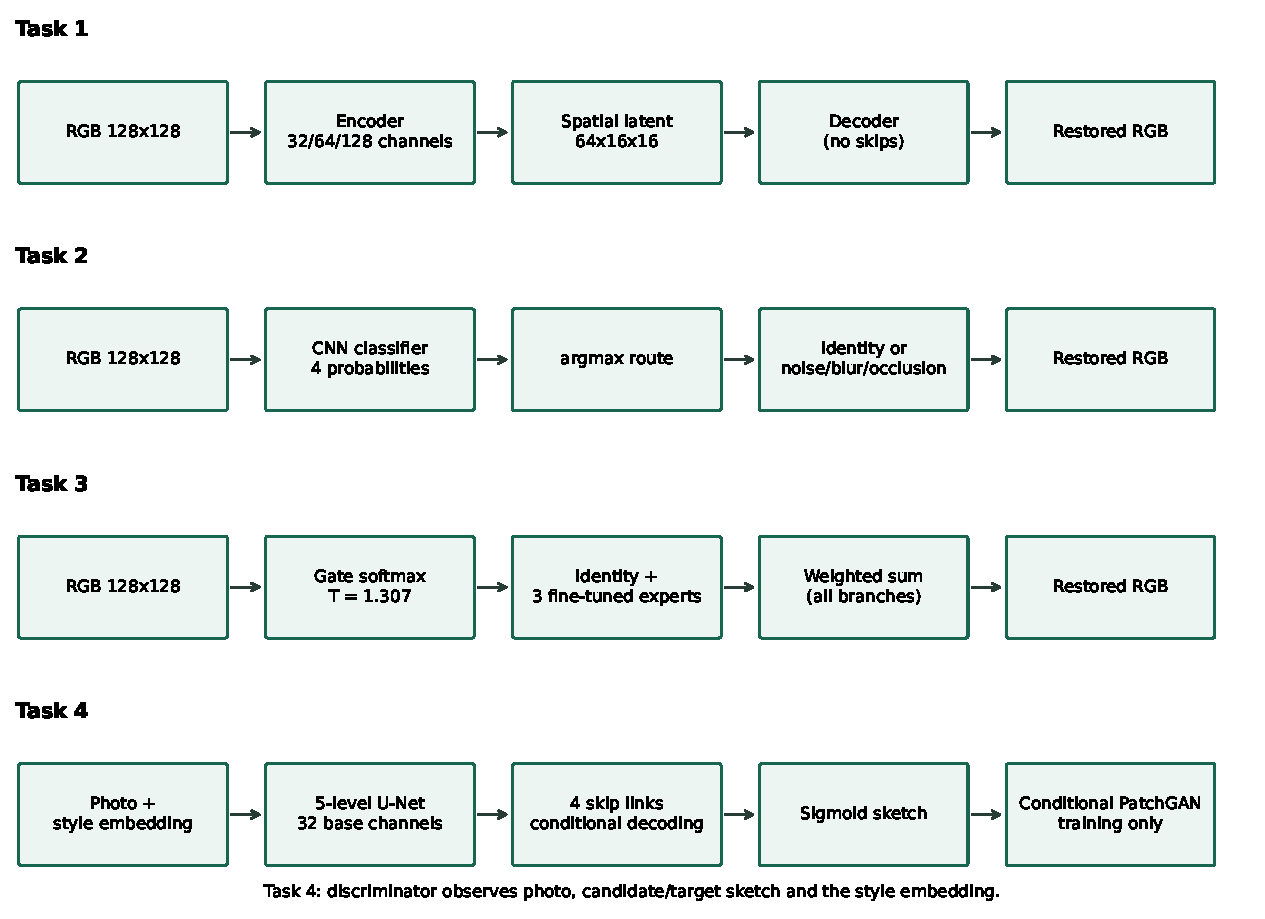
\includegraphics[width=.93\textwidth]{assets/architectures.pdf}\caption{Implemented inference architectures. The Task 4 discriminator is used during training, not deployment. Task 1 has no skips; Task 4 uses paired U-Net skips.}\label{fig:arch}\end{figure*}

\section{Experimental Design and Optimization}
All experiments use seed 42, persistent Optuna TPE studies and median pruning. Training records, curves, checkpoints and result artifacts are logged to MLflow. Checkpoints retain optimizer and RNG states. Resume tests compare uninterrupted and resumed model states; budgets and manifest fingerprints prevent accidentally reusing an incompatible study. Short trials are retrained from scratch for final selection, except Task 3's required Task 2 initialization.

\begin{table}[t]\centering\caption{Recorded studies, including pruned or other non-complete trials. Trial numbers are zero-based.}\label{tab:optuna}\begin{tabular}{lrrr}\toprule Study & Total & Complete & Best trial\\\midrule
T1 & 12 & 8 & 1\\
T2 classifier & 8 & 6 & 2\\
T2 noise & 6 & 5 & 2\\
T2 blur & 6 & 4 & 2\\
T2 occlusion & 6 & 4 & 2\\
T3 & 6 & 5 & 2\\
T4 & 6 & 3 & 1\\
\bottomrule\end{tabular}\end{table}

Task 1 searches learning rate $10^{-4}$--$3\times10^{-3}$, batch $\{16,32,64\}$, latent $\{4096,8192,16384\}$, widths $\{16,32,48\}$, dropout $0$--$.1$ and alpha $.5$--$.95$. The recorded base study has 12 trials with a ten-epoch budget; Run A subsequently increases the selected 8,192 latent to 16,384 while keeping other settings fixed. It is a validation-guided ablation, not the direct unmodified Optuna winner.

Task 2 has eight five-epoch classifier trials and six eight-epoch trials per specialist. Classifier tuning varies rate, width, dropout and weight decay; specialist tuning additionally varies batch size, latent and alpha. Task 3 uses six short warm-up/joint trials varying joint rate $2\times10^{-5}$--$2\times10^{-4}$, temperature $.35$--$1.5$, alpha $.6$--$.95$, classification weight $.01$--$.2$, and balance weight $10^{-4}$--$.02$. Task 4 uses six five-epoch trials varying generator/discriminator rates, width $\{16,32\}$, batch $\{8,16\}$, embedding $\{4,8,16\}$, dropout $0$--$.3$ and L1 coefficient $30$--$150$. Table~\ref{tab:optuna} and Fig.~\ref{fig:trials} record completed studies rather than treating pruned trials as fully trained alternatives.

\begin{figure*}[t]\centering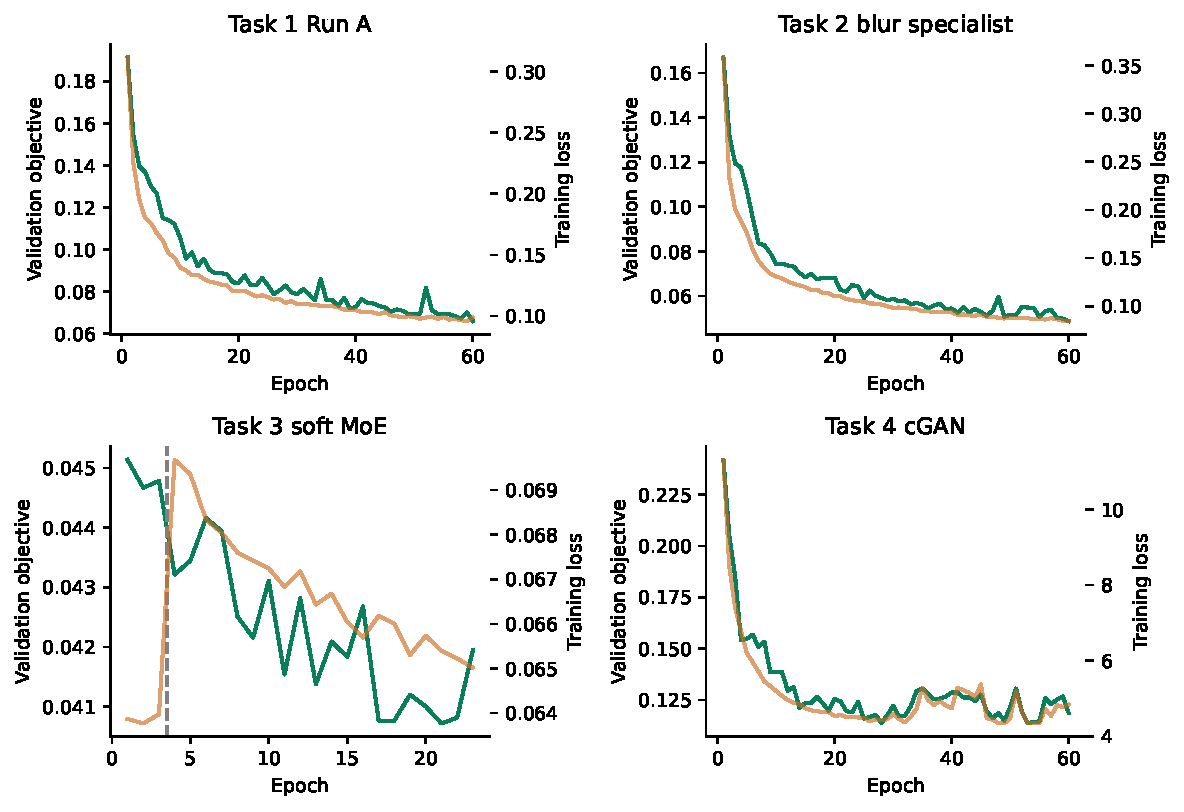
\includegraphics[width=.94\textwidth]{assets/training_curves.pdf}\caption{Final training and validation histories. Green is the fixed validation selection objective; orange is training loss on a separate axis. Their numerical scales differ, so the gap is not a direct generalization-gap measurement. The Task 3 dashed line marks joint fine-tuning.}\label{fig:curves}\end{figure*}
\begin{figure*}[t]\centering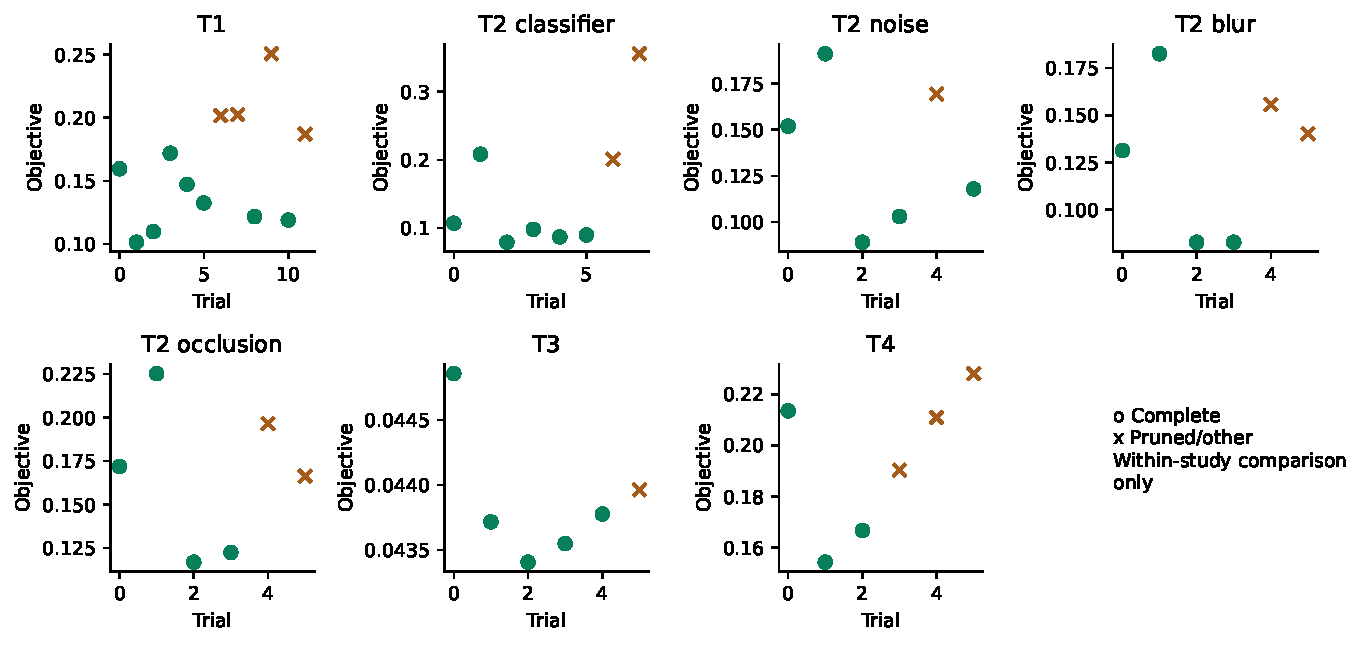
\includegraphics[width=.94\textwidth]{assets/optuna_trials.pdf}\caption{Recorded trial objectives. Completed and pruned/other trials are distinguished. Objectives and epoch budgets differ across studies; values should only be compared within a study.}\label{fig:trials}\end{figure*}
\begin{figure}[t]\centering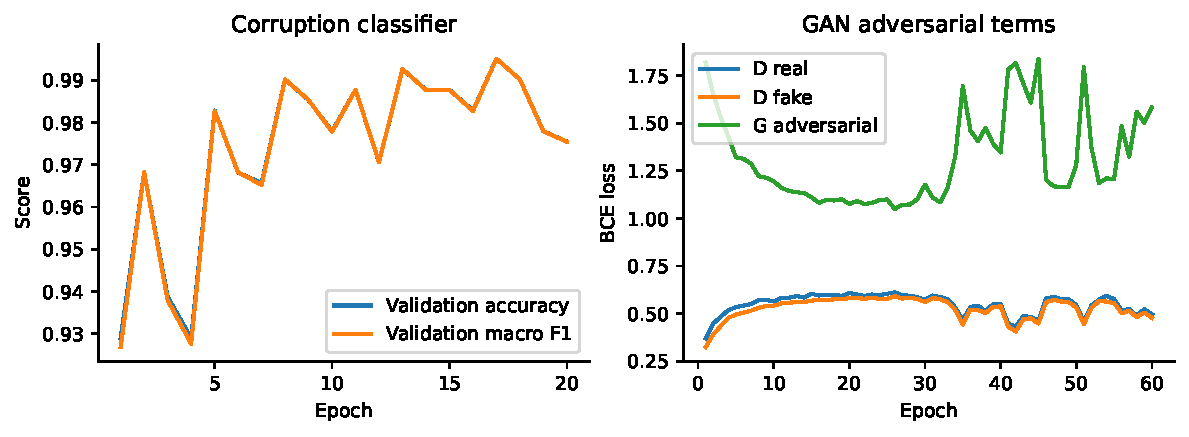
\includegraphics[width=\columnwidth]{assets/classifier_gan_curves.pdf}\caption{Classifier validation scores and separate GAN adversarial losses. GAN loss movement alone does not establish improved visual quality.}\end{figure}

\subsection{Measures and scope}
We report per-image L1, PSNR and SSIM, averaged within each condition/severity. PSNR is $-10\log_{10}(\max(\mathrm{MSE},10^{-12}))$, yielding a finite 120-dB ceiling for exact identity. Classifier accuracy, macro F1 and row-normalized confusion expose routing behavior. Soft gate weights and dominant-class metrics are descriptive: a useful blend need not put the true class first. Sketch scores include an all-white baseline and per-photo pairwise style differences, which measure diversity rather than artistic correctness.

Models are frozen before final test comparison; the release manifest records hashes of the selected models and uploaded archives. The official test photographs were previously evaluated with an older vector baseline, so they cannot be described as completely unseen across the project's history. They were not used for gradient updates or selecting these final candidates. Multiple severity views of one source are correlated; one seed per configuration does not establish significance or repeatability. Training was performed through the GPU-enabled Colab notebooks, but the precise accelerator model is not preserved sufficiently to claim a specific GPU here. Final evaluation records CPU, eight Torch threads and batch 32.

\section{Results and Analysis}
\subsection{Validation-guided decisions}
On the original fixed validation cases, Tasks 1/2/3 attain noise PSNR 26.63/27.66/28.06, blur 26.72/28.13/29.61 and occlusion 21.00/21.74/22.10 dB. Task 3 also improves corrupted groups over its gate-only warm-up. These are validation scores on one sampled condition per photograph, not test severities.

The compression ablation favors Run A over the 8,192-latent baseline for pixel fidelity. In fixed mild/medium/high blur audits, Run A PSNR is 27.98/26.68/24.45 versus baseline 27.59/26.35/24.27. Run B changes alpha to $.5$ while keeping the smaller latent; it slightly improves SSIM but reduces PSNR to 27.39/26.28/24.25. Since A versus B changes both latent and alpha, it does not isolate alpha alone. The baseline-versus-B comparison isolates the configured loss-weight change, within the limitation of one seed.

Mild blur remains a central failure: input PSNR is 33.63 dB, while Tasks 1/2/3 yield 27.98/29.53/32.41. Task 3 improves both PSNR and SSIM over input on only 25 of 408 mild cases, despite recovering much of the loss relative to Task 2. For medium and high blur, Task 3 improves both metrics on 394 and 408 cases respectively. Mean mild identity/blur weights are $.592/.388$; high-blur weights are $.145/.848$. This condition-dependent usage is consistent with preservation-aware blending, not proof of globally optimal routing.

\begin{figure*}[t]\centering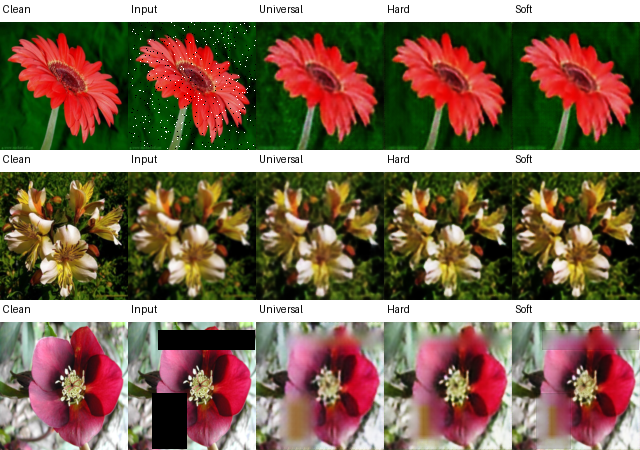
\includegraphics[width=.94\textwidth]{assets/restoration_validation.png}\caption{Paired validation comparisons selected as the first shared filename for each corruption, rather than by metric gain. The clean and input pixels are verified identical across the three source panels. Reconstruction softness and missing-region errors remain visible.}\label{fig:restoration}\end{figure*}

\subsection{Frozen official-test restoration}
\IfFileExists{generated/test_psnr.tex}{
\begin{table*}[t]\centering\caption{Frozen selected-model test PSNR (dB), 6,149 cases per row. Exact identity uses a 120-dB ceiling.}\label{tab:testpsnr}\begin{tabular}{llrrrr}\toprule Condition & Severity & Input & Universal & Hard & Soft\\\midrule
Clean & none & 120.00 & 28.00 & 117.85 & 59.95\\
Noise & low & 19.91 & 27.67 & 28.35 & 28.89\\
Noise & medium & 15.64 & 26.96 & 27.99 & 28.42\\
Noise & high & 12.91 & 25.84 & 27.30 & 27.77\\
Blur & low & 33.69 & 28.04 & 29.67 & 32.41\\
Blur & medium & 27.36 & 26.74 & 28.43 & 29.27\\
Blur & high & 24.47 & 24.49 & 25.51 & 26.10\\
Occlusion & low & 16.82 & 23.86 & 24.52 & 24.78\\
Occlusion & medium & 13.74 & 21.50 & 22.22 & 22.58\\
Occlusion & high & 11.23 & 19.38 & 20.16 & 20.22\\
\bottomrule\end{tabular}\end{table*}
\begin{table*}[t]\centering\caption{Frozen selected-model test SSIM, same 61,490 cases. Higher is better; compare within each condition/severity.}\label{tab:testssim}\begin{tabular}{llrrrr}\toprule Condition & Severity & Input & Universal & Hard & Soft\\\midrule
Clean & none & 1.0000 & 0.8794 & 0.9973 & 0.9990\\
Noise & low & 0.6090 & 0.8678 & 0.8878 & 0.8973\\
Noise & medium & 0.3437 & 0.8431 & 0.8783 & 0.8871\\
Noise & high & 0.2064 & 0.7995 & 0.8599 & 0.8699\\
Blur & low & 0.9639 & 0.8767 & 0.9097 & 0.9488\\
Blur & medium & 0.8485 & 0.8314 & 0.8844 & 0.8983\\
Blur & high & 0.7250 & 0.7293 & 0.7752 & 0.7933\\
Occlusion & low & 0.8593 & 0.8145 & 0.8403 & 0.8832\\
Occlusion & medium & 0.7343 & 0.7526 & 0.7844 & 0.8108\\
Occlusion & high & 0.5487 & 0.6618 & 0.7030 & 0.7143\\
\bottomrule\end{tabular}\end{table*}
\begin{table}[t]\centering\caption{Test mean L1. Corrupted conditions average their three equally supported severity groups; clean uses its single view.}\resizebox{\columnwidth}{!}{\begin{tabular}{lrrrr}\toprule Condition & Input & Universal & Hard & Soft\\\midrule
Clean & 0.00000 & 0.02873 & 0.00058 & 0.00105\\
Noise & 0.04334 & 0.03317 & 0.02878 & 0.02721\\
Blur & 0.02691 & 0.03448 & 0.02882 & 0.02469\\
Occlusion & 0.08624 & 0.05015 & 0.04489 & 0.04042\\
\bottomrule\end{tabular}}\end{table}
The final comparison evaluates every official test photograph under all ten recorded views. Classifier accuracy is \TestAccuracy{} and macro F1 is \TestFOne{}. Tables~\ref{tab:testpsnr} and~\ref{tab:testssim} provide the full severity comparisons; the accompanying per-image CSV includes L1, oracle scores, paired improvement counts, class probabilities and soft branch weights. No further model selection follows these results.
\begin{figure}[t]\centering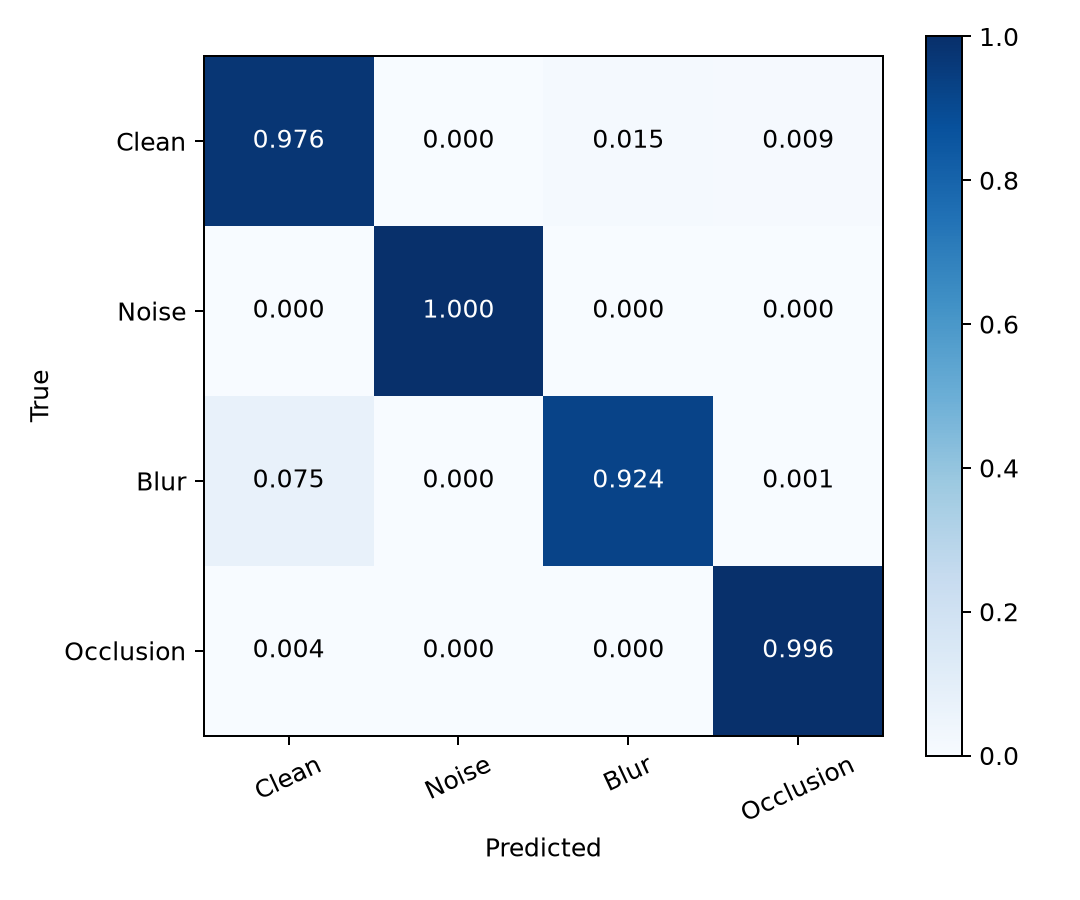
\includegraphics[width=\columnwidth]{assets/confusion_matrix.png}\caption{Test hard-router confusion. Rows are true conditions and columns predictions. Test support is 6,149 clean and 18,447 for each corrupted class.}\label{fig:confusion}\end{figure}
\begin{figure}[t]\centering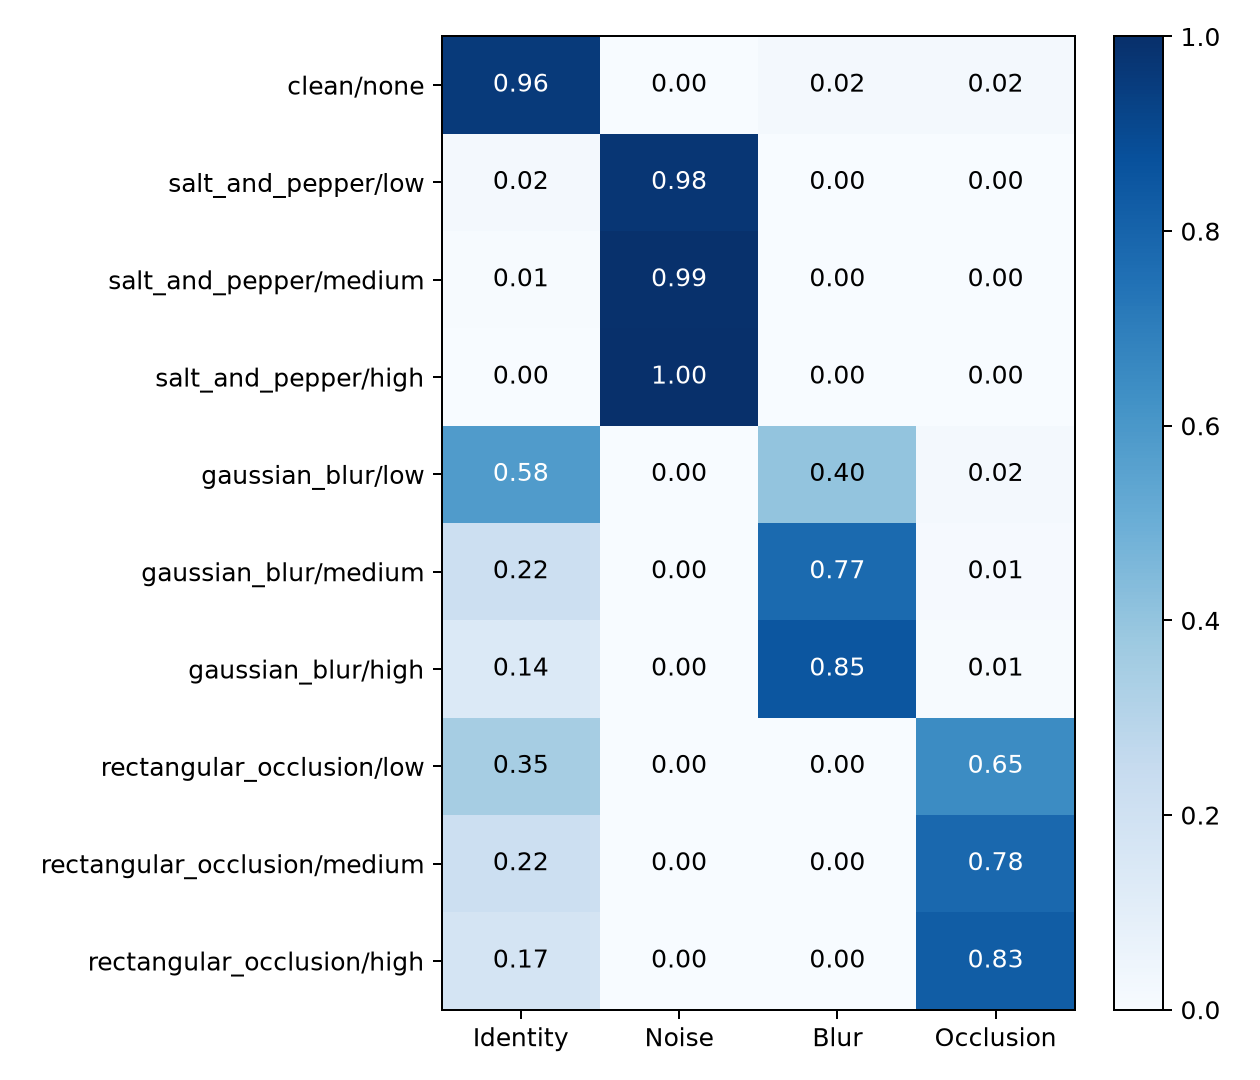
\includegraphics[width=\columnwidth]{assets/routing_heatmap.png}\caption{Test mean soft branch weights by condition/severity. Identity contributions and branch preference should be considered alongside reconstruction metrics.}\label{fig:weights}\end{figure}
The soft mixture improves mean PSNR and SSIM over hard routing in all nine corrupted test severity groups. For mild blur, it still reduces PSNR from 33.69 to 32.41 dB and improves both input metrics on only 305/6149 cases. Medium and high blur improve both metrics on 5966/6149 and 6132/6149. Mean identity/blur weights shift from 0.579/0.400 at low blur to 0.139/0.854 at high blur. These test findings support the validation interpretation while preserving the mild-blur limitation.

Hard routing correctly identifies 6004 of 6149 clean views. Its largest confusion is blur classified as clean (1391 cases across severities). Only 221 wrong-route cases lose PSNR relative to oracle routing; bypassing a weak mild-blur expert can accidentally improve PSNR. Thus classification accuracy and restoration quality are related but not interchangeable. The soft mixture changes most clean images slightly, whereas hard routing usually returns them exactly. Soft clean mean SSIM exceeds hard clean SSIM here despite lower clean mean PSNR, because the hard router has occasional clean-image dispatch failures and an identity ceiling. These are descriptive single-seed measurements, not statistical significance tests.

\begin{figure}[t]\centering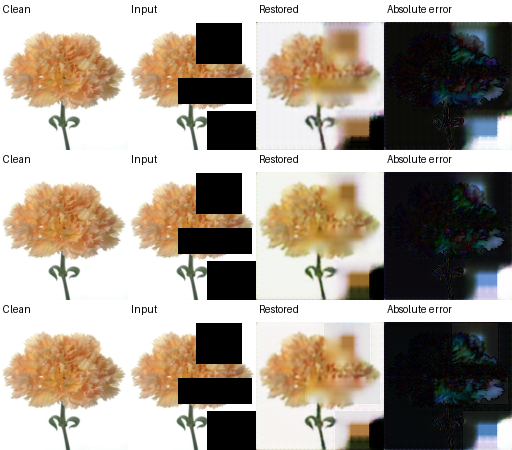
\includegraphics[width=\columnwidth]{assets/test_failures.png}\caption{Largest-L1 test candidate for universal, hard and soft reconstruction (top to bottom). Each model's failure is selected separately and may depict a different source; this is not a paired model ranking.}\end{figure}
}{\textbf{Final restoration test evaluation is pending. No validation score is substituted as a test result.}}

Clean identity can dominate overall PSNR: Task 2 may pass images exactly, while a soft mixture slightly changes them. On the clean validation severity audit, Task 3 mean identity weight is $.959$, SSIM $.998884$ and L1 $.000997$, but one of 408 cases falls below 30 dB. Consequently, clean preservation and corrupted restoration are discussed separately. Scores also cannot show that an occluded petal was reconstructed as its original unseen detail; plausible filling is a weaker claim than exact recovery.

\subsection{Sketch generation}
\begin{table}[t]\centering\caption{Task 4 official-test scores, 356 photographs per style; PSNR in dB.}\label{tab:sketch}\resizebox{\columnwidth}{!}{\begin{tabular}{lrrrr}\toprule Style & L1 & SSIM & PSNR & Blank SSIM\\\midrule
Fine Pencil & 0.0347 & 0.9020 & 24.81 & 0.2827\\
Technical Ink & 0.1630 & 0.5272 & 8.31 & 0.1400\\
Tonal Charcoal & 0.0376 & 0.8183 & 14.87 & 0.2910\\
\bottomrule\end{tabular}}\end{table}
Test style results in Table~\ref{tab:sketch} closely track validation: pencil SSIM $.90195$ versus $.90273$, ink $.52724$ versus $.52518$, charcoal $.81826$ versus $.81492$. Each style beats the blank-white baseline on average, so the average quality is not explained by blank output alone. Generated test pairwise L1 is $.42354$ for pencil/ink, $.17705$ for pencil/charcoal and $.41959$ for ink/charcoal, compared with target differences $.44066/.18402/.42881$. These aggregate separations and the inspected panels show distinct styles, while ink remains the weakest target match.

\begin{figure}[t]\centering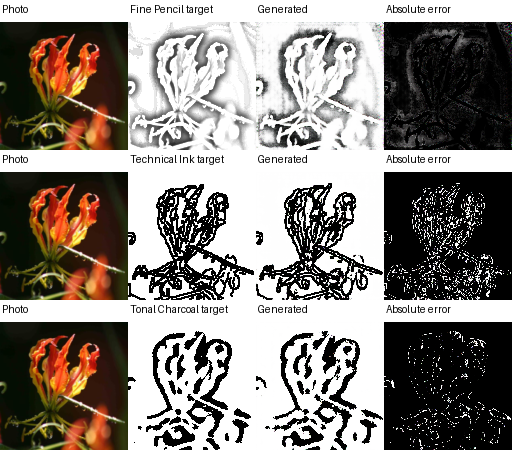
\includegraphics[width=\columnwidth]{assets/sketch_validation.png}\caption{One validation photograph under pencil, ink and charcoal conditioning. Each row shows photo, synthetic target, generated sketch and absolute error.}\end{figure}
\begin{figure}[t]\centering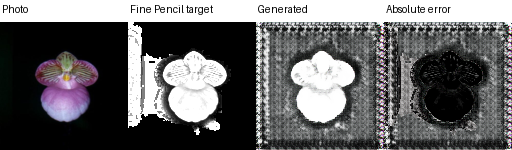
\includegraphics[width=\columnwidth]{assets/pencil_failure.png}\\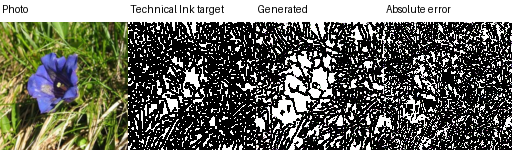
\includegraphics[width=\columnwidth]{assets/ink_test_failure.png}\caption{Pencil validation failure with visible grid artifacts and ink test failure with dense contour mismatch. Artifact causes were not isolated; architecture, target statistics and optimization remain hypotheses.}\end{figure}
The strong pencil mean conceals a conspicuous grid pattern on validation source 5100. Ink test failures are concentrated among dense edge targets, including source 5229. Small contour displacements can create substantial pixel disagreement in binary targets, but this observation is not a controlled proof of the error's cause. Images outside the flower domain may behave differently; the system is not validated as a general portrait sketch generator.

\section{Application, Export and Deployment}
The browser application has Universal Restoration, Hard-Routed Restoration, Soft MoE Restoration and Object-to-Sketch workspaces. React/Tailwind collects either an upload or a prepared sample, exposes corruption controls for restoration and a categorical selector for sketches, and displays PNG results with a download link. FastAPI validates image decoding, upload size (5 MB), parameter ranges and source selection, then preprocesses to the training convention. Model sessions are cached and inference uses ONNX Runtime CPU. Uploaded already-corrupted images have no known clean target; reference/error maps are displayed only for a sample or simulated corruption. Sketch photos are not presented as sketch ground truth.

Seven fixed-batch ONNX graphs are installed: universal, classifier, three specialists, soft pipeline and sketch generator. Metadata hashes enforce artifact identity. Independent parity checks cover 16 validation inputs for universal and soft pipelines, 16 for each Task 2 component, and all 786 Task 4 validation pairs. Restoration output errors are approximately $5\times10^{-7}$; Task 4 accumulates larger but small differences through instance normalization. Maximum Task 4 error is $.000146985$ on $[0,1]$, or $.0375$ of an 8-bit level. Re-exporting did not reduce it. We retain the graph and document a fixed $.0002$ absolute error budget and $.0001$ relative tolerance; all validation pairs pass. This numerical tolerance revision does not change learned image quality.

\begin{figure}[t]\centering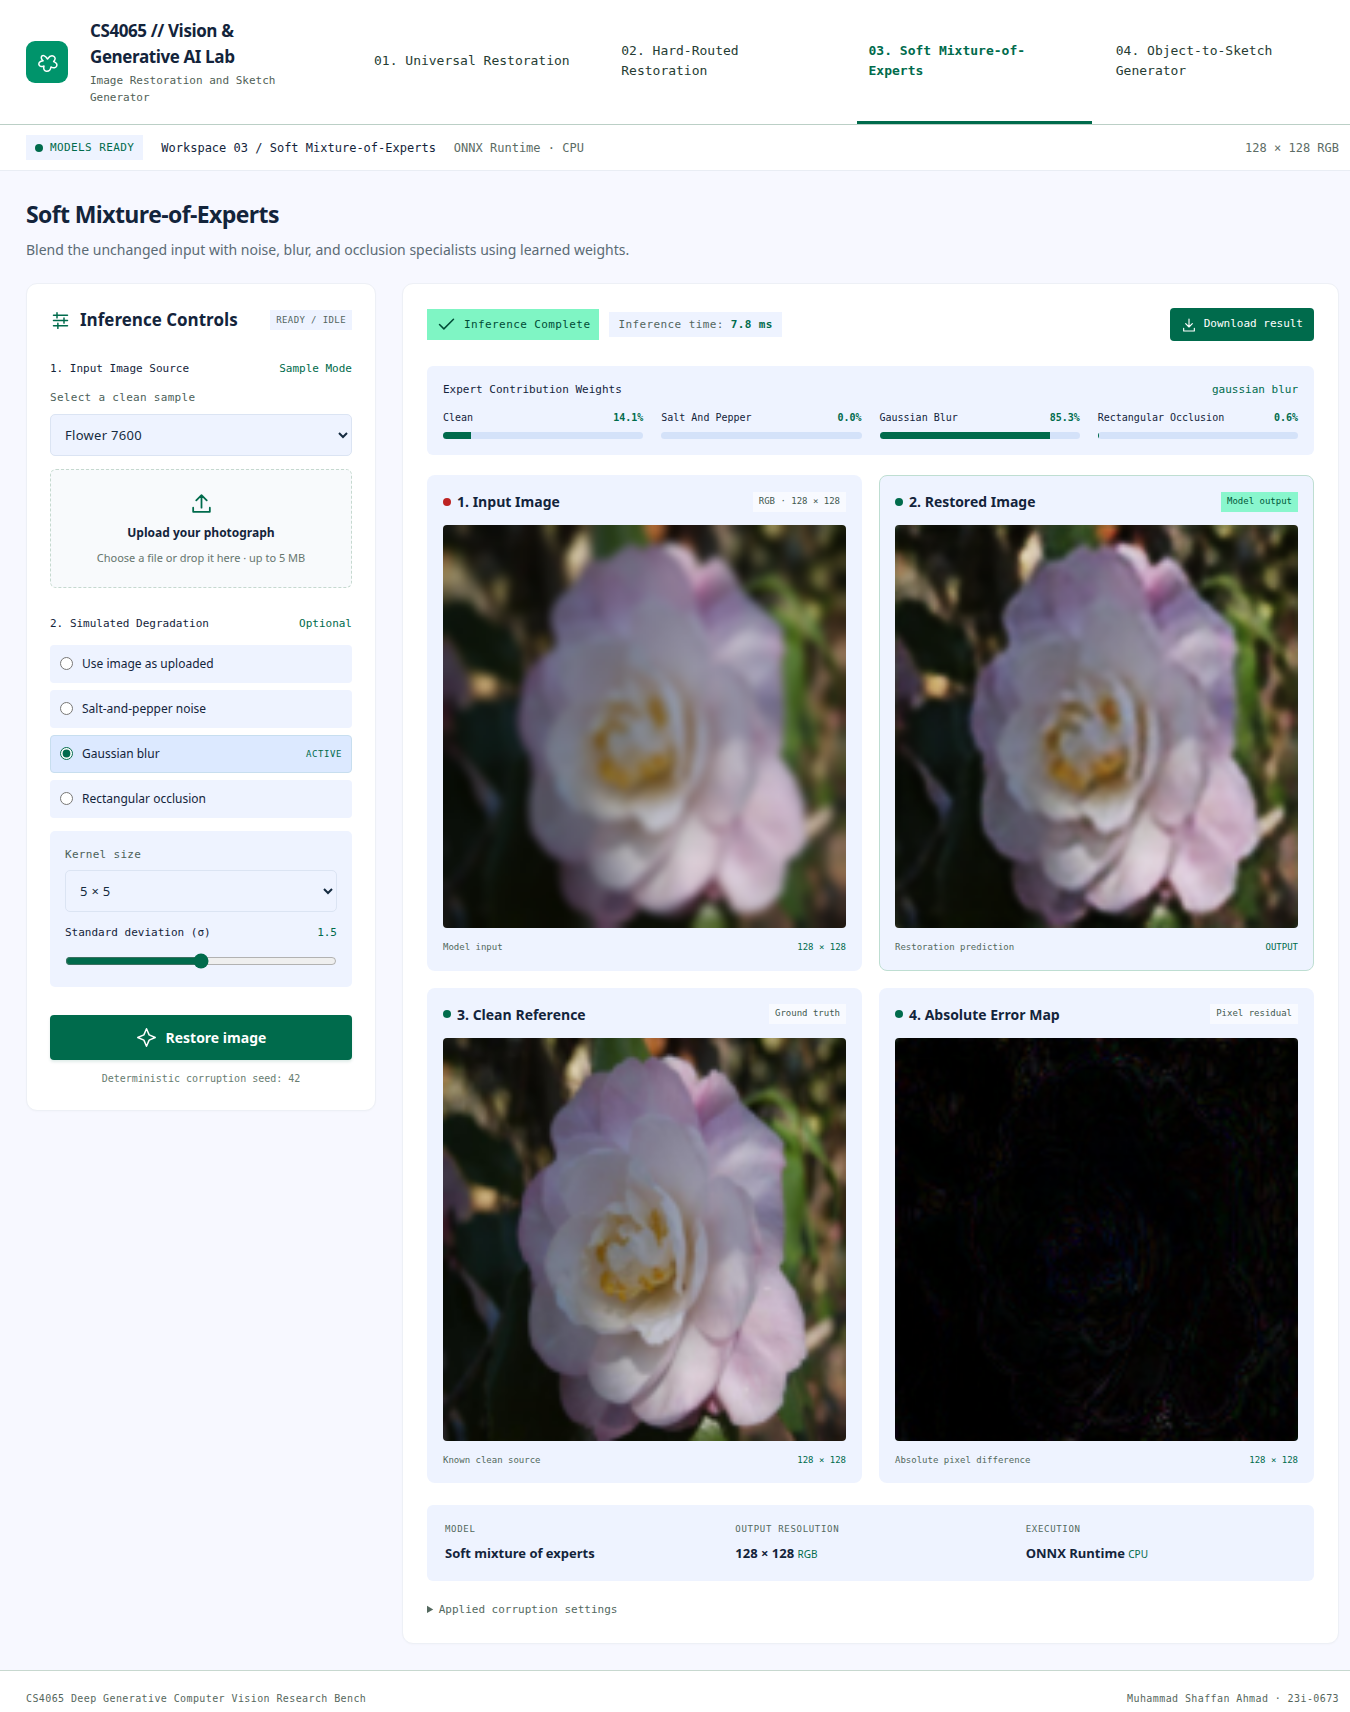
\includegraphics[width=\columnwidth]{assets/app_desktop.png}\caption{Integrated production UI: soft routing weights, input, reconstruction, known reference, error map and download. The displayed latency is one inference, not a throughput benchmark.}\label{fig:ui}\end{figure}
Both Docker images build successfully. The frontend Nginx container serves the production bundle and proxies $/api$ to FastAPI. Model and data volumes are read-only. Container startup and all 15 sample inference combinations pass through the Docker frontend. Verification uses host ports 18081/18082 to avoid an unrelated existing 8080 service; defaults remain 8080/8000 and can be overridden. The evaluator's command is \texttt{docker compose up --build} after obtaining models and preparing data. Production browser checks exercise four workspaces, three sketch styles, routing displays and download links. Desktop/mobile screenshots at widths 1365/390 have no horizontal overflow. All 23 automated Python tests pass. These checks do not establish physical-device testing or public-hosting reliability.

\section{Limitations and Conclusion}
Specialization improves the universal baseline on the recorded corrupted validation groups, and soft blending further improves them while preserving more lightly corrupted information. Neither approach solves mild-blur preservation or unseen occlusion detail. The conditional GAN learns distinct algorithmic styles with unequal fidelity; ink contours and localized grid artifacts remain material limitations. Additional seeds, broader domains, real degradation and human sketch judgments would be required for stronger generalization claims.

This assignment delivers a controlled data foundation, four trained systems, tracked search evidence, ONNX inference and a verified containerized application. Results are interpreted per condition and style instead of inflated aggregate scores. Account-dependent design/publication artifacts are explicitly identified below; a working application alone does not satisfy every submission requirement.

\section*{Artifact Availability and Submission Evidence}
Repository destination supplied by the author:\\
\url{https://github.com/M-Shaffan-Ahmad/GENAI_ImageSketchGenerator}.\\
Source and frozen trained artifacts are published in the author's public repository. Signed-out access and the model package SHA-256 were verified. Model download: \ModelDownloadLink. Demonstration video: \DemoVideoLink. Stitch evidence: \StitchEvidenceStatus.

The earlier React UI preceded the supplied Google Stitch export. On October 4, 2026, the author supplied the export, and the app was revised to follow its lab header, emerald/pale-blue palette, workspace navigation, control cards and result panels. Original exported HTML, screenshots and design notes are preserved with hashes in \texttt{report/stitch/}. The export's generation date and original prompt were not independently available. Prototype GPU, diffusion, resolution and fidelity placeholders were replaced with actual CPU ONNX inference, 128-pixel outputs and measured latency. Figure~\ref{fig:stitch} is the supplied design, while Figure~\ref{fig:ui} shows the working application. The author supplied the uploaded demonstration link above. Final author review and Classroom submission remain.

\begin{figure}[t]\centering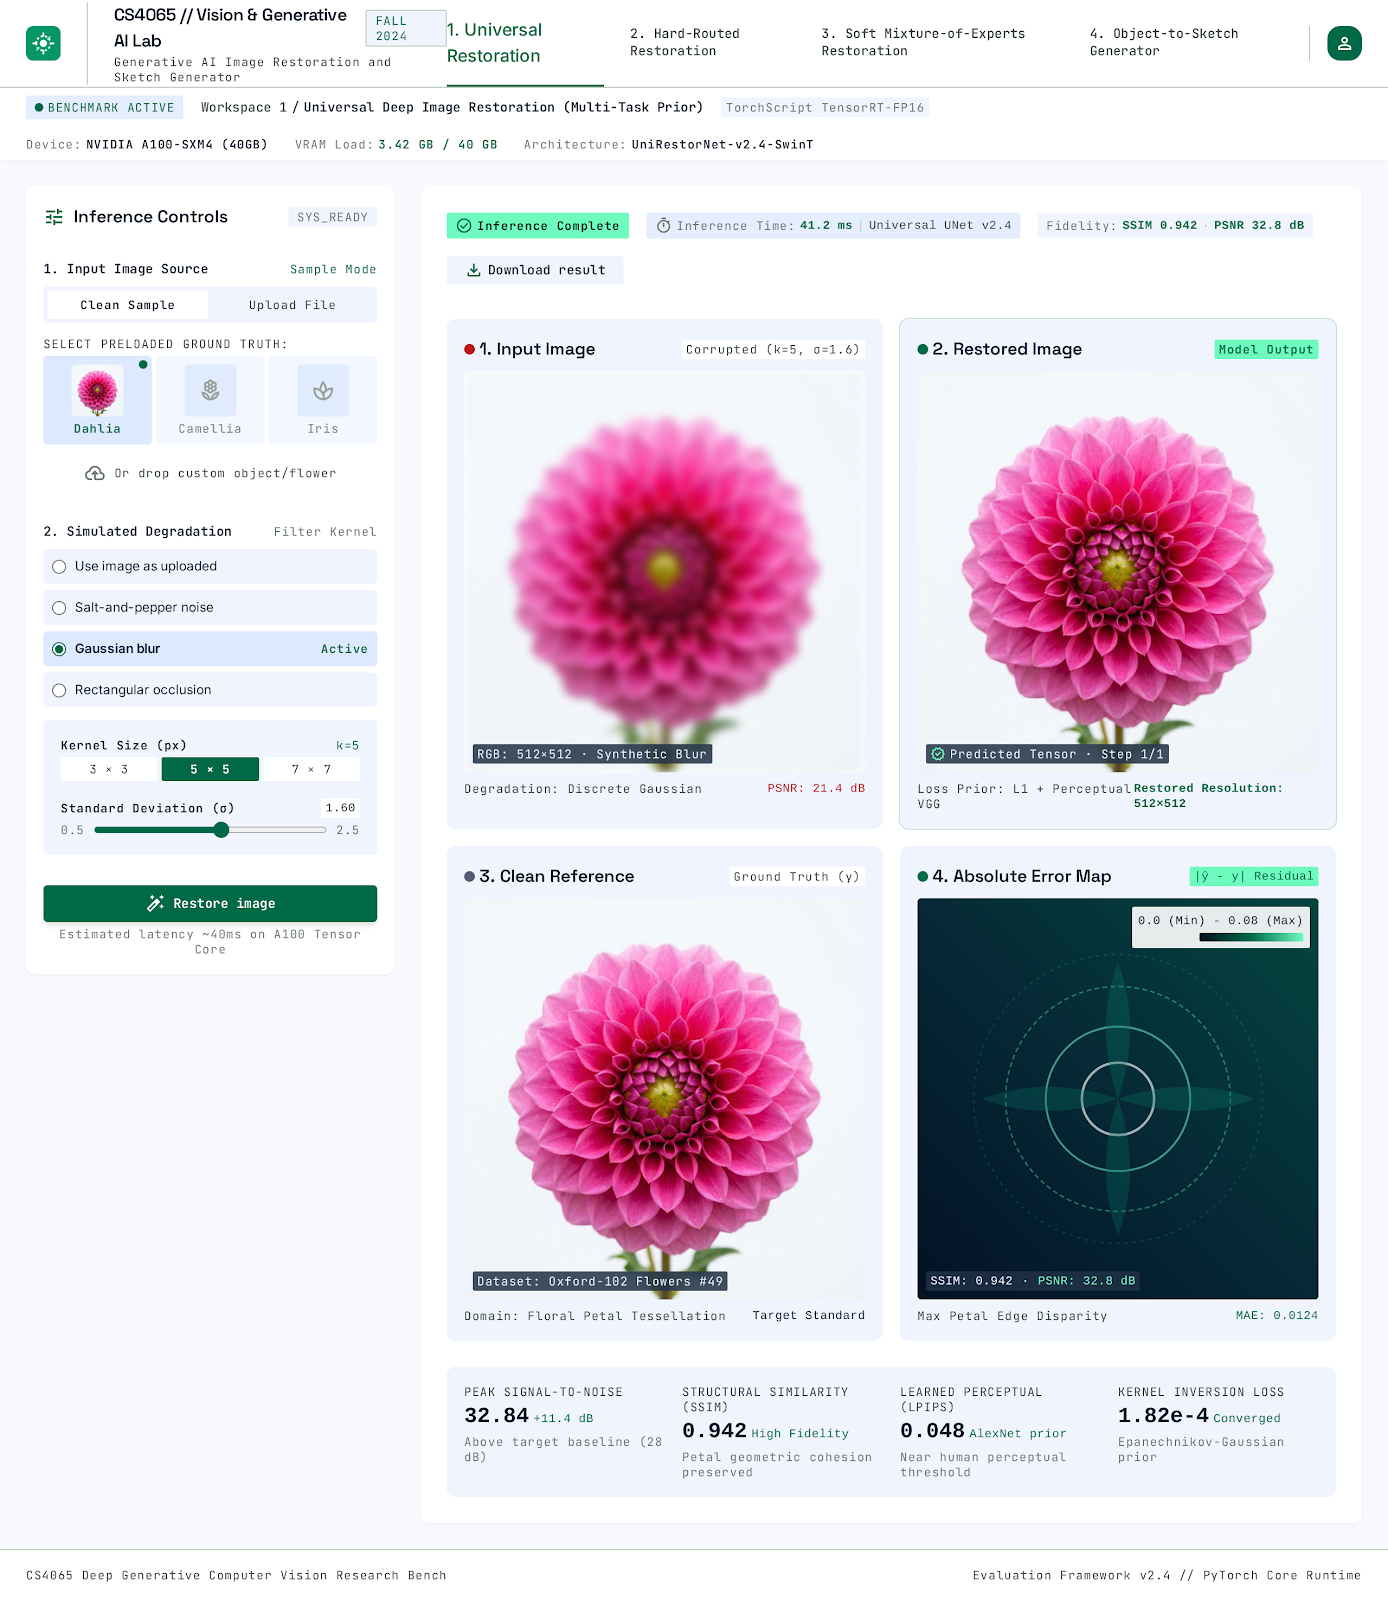
\includegraphics[width=\columnwidth,height=.50\textheight,keepaspectratio]{assets/stitch_universal.png}\caption{Original universal-restoration screen from the author's supplied Stitch export. Its example images, GPU/runtime and fidelity values are design placeholders, not measured results from our trained models.}\label{fig:stitch}\end{figure}

\appendices
\section{AI Assistance and Verification}
The author directed the project workflow, ran the Colab training workflows and supplied their result archives, inspected the outputs and requested further investigation of blur preservation and sketch quality. The author also supplied the Google Stitch export and recorded and uploaded the demonstration. These activities were performed alongside AI assistance; AI use does not replace the author's responsibility to understand and verify the submitted system.

OpenAI Codex was used for assistance with implementation and debugging of data preparation, PyTorch training/evaluation/export code, React/FastAPI integration, interpretation of experiment outputs, report drafting and packaging. Representative requests included fixing the data foundation, implementing Tasks 1--4, investigating blurred reconstructions, preparing Colab workflows and integrating the trained models. These are summaries of the iterative requests, rather than a complete prompt transcript.

Verification evidence includes executed manifest/source-hash checks, grouped-split and corruption tests, model/gradient tests, resume-equivalence checks, checkpoint provenance, ONNX graph checks and numerical parity, actual API inference, production browser checks and Docker build/start checks. Corrections addressed compression assumptions, separated the fixed validation-selection objective from tunable training loss, documented clean/mild-blur preservation failures and recorded the GAN's original export-tolerance failure before applying a stated numerical error budget. The reported final results were calculated from the frozen selected models rather than substituted from earlier baselines.

Research references were checked against primary paper or institutional sources. Reported model metrics come from the project's evaluation artifacts, not from cited papers or AI estimates. The author remains responsible for reviewing the report, understanding the loss formulations, data splits, routing, code and failure cases, and explaining or modifying the system during evaluation.

\begin{thebibliography}{6}
\bibitem{flowers}M.-E. Nilsback and A. Zisserman, ``Automated flower classification over a large number of classes,'' in \emph{Proc. Indian Conf. Computer Vision, Graphics and Image Processing}, 2008. [Online]. Available: \url{https://www.robots.ox.ac.uk/~vgg/publications/2008/Nilsback08/nilsback08.pdf}
\bibitem{vincent}P. Vincent, H. Larochelle, Y. Bengio, and P.-A. Manzagol, ``Extracting and composing robust features with denoising autoencoders,'' in \emph{Proc. ICML}, 2008, pp. 1096--1103. doi: 10.1145/1390156.1390294.
\bibitem{ssim}Z. Wang, A. C. Bovik, H. R. Sheikh, and E. P. Simoncelli, ``Image quality assessment: From error visibility to structural similarity,'' \emph{IEEE Trans. Image Process.}, vol. 13, no. 4, pp. 600--612, 2004. doi: 10.1109/TIP.2003.819861.
\bibitem{moe}N. Shazeer et al., ``Outrageously large neural networks: The sparsely-gated mixture-of-experts layer,'' in \emph{Proc. ICLR}, 2017. [Online]. Available: \url{https://arxiv.org/abs/1701.06538}
\bibitem{pix2pix}P. Isola, J.-Y. Zhu, T. Zhou, and A. A. Efros, ``Image-to-image translation with conditional adversarial networks,'' in \emph{Proc. CVPR}, 2017, pp. 1125--1134. [Online]. Available: \url{https://arxiv.org/abs/1611.07004}
\bibitem{optuna}T. Akiba, S. Sano, T. Yanase, T. Ohta, and M. Koyama, ``Optuna: A next-generation hyperparameter optimization framework,'' in \emph{Proc. KDD}, 2019, pp. 2623--2631. doi: 10.1145/3292500.3330701.
\end{thebibliography}
\end{document}
